\documentclass[letterpaper, reqno,11pt]{article}
\usepackage[margin=1.0in]{geometry}
\usepackage{color,latexsym,amsmath,amssymb,graphicx,float,listings,tikz}
\usepackage{hyperref}

\hypersetup{
colorlinks=true,
linkcolor=magenta,
filecolor=magenta,
urlcolor=cyan,
}

\graphicspath{ {images/} }

\tikzstyle{vertex}=[shape=circle, minimum size=2mm, fill, draw, inner sep=0]

\begin{document}
\pagenumbering{arabic}
\title{Math 443 Homework 5}
\date{01/03/23}
\author{Xander Naumenko}
\maketitle

{\medskip\noindent\bf Question 1.} Let $k$ be a positive integer, and let $A_1,A_2$ be two copies of $K_{k+1}$ (the example also works for $K_k$, but it's easier to show minimality this way). Let $G_k$ be created by taking a new vertex, $v$, and connecting it to $k$ vertices in each of $A_1,A_2$. Clearly $\kappa(G_k)=1$ since if $v$ is removed $G_k$ gets separated into $A_1,A_2$ as components. To see that $\lambda(G_k)\leq k$, note that by removing all edges between $v$ and $A_1$ results in a disconnect graph, which is an edge set of size $k$. 

To see why this is a minimum edge cut, let $E\subset E(G_k)$ s.t. $|E|<k$ (since $E$ is an edge set the $\left|  \right| $ syntax denotes size of set, not number of vertices). Then $E$ couldn't have removed all the edges between $A_1$ and $v$, since there are $k$ edges between them. By symmetry the same applies for $A_2$ and $v$. $A_1-E$ and $A_2-E$ are still connected since they are both copies of $K_{k+1}$. Since $A_1$ and $A_2$ are internally connected and $v$ is still connected to both after the removal of $E$, the whole graph is still connected and $\lambda(G_k)\geq k$. Thus $\lambda(G_k)=k$ and $\kappa(G_k)=1$ as required. 

{\medskip\noindent\bf Question 2a.} The statement is true. Let $E$ be a separating edge set of $G$, and let $A$ be a smallest resulting component of $G-E$. Clearly $|A|\leq \frac{n}{2}$ since it the smaller of at least two components whose total vertices is $n$. Note that $| |A| |\leq K_{|A|}=|A|(|A|-1)$. Also note that the total number of edges of the vertices of $A$ in $G$ is $|A|\cdot \delta(G)$. The difference between these numbers is at least the number of vertices taken away by $E$, i.e. $|E|\geq |A| \delta(G)-|A|(|A|-1)=|A|\left( \delta(G)-|A|+1 \right) $. This is a downward parabola in $|A|$, so from calculus its minimum must lie on one of the two endpoints, i.e. $|A|=1$ or $|A|=\frac{n}{2}$. These two values are: 
\[
|E|\geq \delta(G)-1+1=\delta(G)
.\]
\[
|E|\geq \frac{n}{2}(\delta(G)-\frac{n}{2}+1)\geq \delta(G)
.\]
We conclude that $\lambda(G)\geq \delta(G)$. In class we also proved that $\lambda(G)\leq \delta(G)$, so these two inequalities together tell us that $\lambda(G)=\delta(G)$ as required. $\square$

{\medskip\noindent\bf Question 2b.} The statement is false. As a counterexample let $k\geq 3$ and consider two copies of $K_k$, $A_1,A_2$. Form $G$ by adding two vertices $v_1,v_2$ connected to all vertices in $A_1,A_2$. Each vertex in $A_1,A_2$ has $k-1$ neighbors from the complete graph as well as $v_1,v_2$ for a total of $k-1+2=k+1$. $v_1,v_2$ each have $2k$ neighbors since their connected to each vertex in $A_1,A_2$. The total vertices is $2k+2$, so $\delta(G)=k+1\geq \frac{|G|}{2}$. We can disconnect the graph by removing $v_1,v_2$, so $\kappa=2$ (it clearly can't be less than that). Let $E$ be an edge set with $|E|\leq 2$. $A_1$ remain connected in $G-E$ since it is $k\geq 3$ complete, and there is at least one edge from $A_1$ to $v_1$ and $v_2$ in $G-E$, since there were at least $3$ edges before and $E$ removed at most 2. By symmetry the same is true for $A_2$, so all 4 of $A_1,A_2,v_1,v_2$ are internally connected and connected together. Thus $E$ is not an edge cut, so $\lambda(G)>2$ and $\lambda(G)\neq \kappa(G)$.  

{\medskip\noindent\bf Question 3.} The statement is not true. Consider the following graph $G$: 

\begin{center}
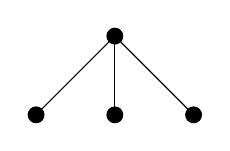
\begin{tikzpicture}
\draw (0,0)node[vertex]{};
\draw (1,0)node[vertex]{};
\draw (2,0)node[vertex]{};
\draw (1,1)node[vertex]{};
\draw (0,0)--(1,1);
\draw (1,0)--(1,1);
\draw (2,0)--(1,1);
\end{tikzpicture}
\end{center}

The three blocks are three copies of $K_2$, and they are each connected to each other since they each share a vertex, so this is $\mathcal{G}$: 

\begin{center}
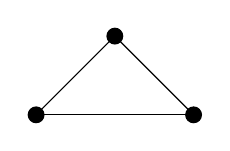
\begin{tikzpicture}
\draw (0,0)node[vertex]{};
\draw (2,0)node[vertex]{};
\draw (1,1)node[vertex]{};
\draw (0,0)--(1,1);
\draw (2,0)--(1,1);
\draw (0,0)--(2,0);
\end{tikzpicture}
\end{center}

This obviously isn't a tree since it contains a cycle, so we're done and the statement is false. 

{\medskip\noindent\bf Question 4a.} The statement is true. Let $v\in G[\mathcal{E}]$. Let $x,y\in G[\mathcal{E}]-v$. Let $C$ be a cycle in $G[\mathcal E]$ containing $x,y$ (this exists since you can choose any two edges attached to $x,y$ and they're guaranteed to share a cycle). Let $P$ be a path along $C$ that doesn't include $v$, since there are two options (each way around $C$) this will always exist. Then $x,y$ are connected in $G[\mathcal{E}]-v$ through $P$. This works for any $v$, so there are no cut vertices in $G[\mathcal{E}]$ so it is nonseparable. $\square$

%\includegraphics[width=0.015\textwidth]{Epsilon}

{\medskip\noindent\bf Question 4b.} The statement is true. By was of contradiction suppose it wasn't true, i.e. suppose that $\exists e=xy\in E(G)$ s.t. $x,y\in V(G[\mathcal E])$ and $e \not\in \mathcal E$. Let $e_x,e_y$ be two edges in $\mathcal E$ with one endpoint on $x,y$ respectively. Since they are related by $R$ there exists a cycle $C$ in $G[\mathcal E]$ that contains both of them. If $e\in C$ then it would be in $\mathcal E$, a contradiction, so assume it isn't. $C$ passes through $e_x$ and $e_y$, so split it into two component paths, both starting at $x$ and ending at $y$ and merge one of them with $e=xy$. The resulting cycle contains $e$ and other edges of $\mathcal E$, so $e\in \mathcal E$. However this contradicts our assumption it wasn't, so $G[\mathcal E]$ must have been an induced subgraph of $G$. $\square$

{\medskip\noindent\bf Question 4c.} The statement is true. We will use proof by contradiction. From part a, $G[\mathcal E]$ is nonseparable, so the only way $G[\mathcal E]$ could not be a block is if it isn't maximal. By way of contradiction suppose that $\exists B\subset G, v\in G, v\notin G[\mathcal E]$ s.t. $B$ is nonseparable and $V(G[\mathcal E])\subset V(B), v\in B,$. It is asserted that there exists paths $P_1,P_2$ from $v$ to $G[\mathcal E]$ in $B$ with the endpoints of $u_1,u_2\in G[\mathcal E], u_1\neq u_2$. At least one path $P_1$ must exist for $v$ and $G[\mathcal E]$ to be connected, and since removing $u_1$ shouldn't disconnect $G[\mathcal E]+v$ a second path must exist with a different endpoint in $G[\mathcal E]$. Choose $P_1,P_2$ in such a way that $u_1,u_2$ are their only member in $G[\mathcal E]$. Consider the first common ancestor between $P_1$ and $P_2$ starting from $u_1,u_2$, call it $x$. $G[\mathcal E]$ is connected so there exists a path in it between $u_1$ and $u_2$, call it $P_3$. Then $u_1P_3u_2P_1xP_2u_1$ is a cycle in $G$ containing an edges not in $G[\mathcal E]$, namely the edges of $P_1,P_2$ before $x$. This is impossible since we assumed $G[\mathcal E]$ was formed by the entire equivalence class, so it must be that $G[\mathcal E]$ is a block of $G$. $\square$

{\medskip\noindent\bf Question 4d.} The statement is true. Suppose by contradiction that it wasn't, i.e. suppose there exists a block $B$ of $G$ and $e_1=xy, e_2=uv\in E(G)$ s.t. $e_1$ and $e_2$ share no common cycle. Additionally choose $e_1,e_2$ such that the distance between $x,u$ is minimal. It can't be that $e_1$ and $e_2$ are adjacent, since otherwise you could delete their shared vertex, find a path between the remaining two (guaranteed by $B$'s nonseparability) and you combine this path with $e_1e_2$ to make a cycle. Therefore there exists a vertex $z$ such that $xz\in E(B)$ and $xz$ is in the minimal path between $x$ and $u$, $z\neq x,y,u,v$. $z$ is strictly closer to $u$ than $x$, so by the minimal choice of $e_1,e_2$, $xz$ and $e_2=uv$ share a common cycle, call it $C$. Define $P_1,P_2$ to be the two ways of going from $x$ to $v$ on $C$ (one of them contain both $uv$ and $xz$). 

Next by the nonseparability of $B$, there exists a path $P$ from $y$ to $v$ s.t. $x\not\in  P$. If $P$ doesn't intersect $C$, then assume $u\in P_1$ and consider the path $xyPvP_1$, this forms a cycle with $xy$ and $uv$ since $uv\in P_1$ which contradicts our assumption that $e_1,e_2$ don't share any. 

If instead $P$ intersects $C$, WLOG assume it intersects $P_1$ (in this specific case we're not assuming $v\in P_1$ anymore, so $P_1,P_2$ are arbitrary). Define the intersection vertex $w$ to be the shared vertex between $P$ and $P_1$ closest along $P$ to $y$, and define $P_1'\subset P_1$ to be the path from $w$ to $v$ and $P'\subset P$ to be the path from $y$ to $w$. Note that $||P_1||\geq 1$ since $w\neq v$ (although it might be $u$), so if $u\in P_1$ then $u\in P_1'$ since $u$ is adjacent to $v$ in $C$. Then the we can form a cycle $xyP'wP_1'vP_2x$. Since one of $P_1',P_2$ contain $u$ by $C$'s definition, this cycle we've constructed has both $xy$ and $uv$ as edges which contradicts our assumption that there was no such common cycle. Thus are assumption must have been wrong and $E(B)$ is an equivalence class of $G$. $\square$

% {\medskip\noindent\bf Question 4d.} The statement is true. Let $B$ be a block of $G$ and $e_1=xy, e_2=uv\in E(B)$. Since $B$ is nonseparable by definition, by theorem 5.7 there exist cycles $C_1$ and $C_2$ such that $x\in C_1,u\in C_1$ and $y\in C_2, v\in C_2$. 

{\medskip\noindent\bf Question 5.} Let $v$ be a cut vertex of $G$. Since it is a cut vertex $d(v)\geq 2$. Let two of its neighbors be $x$ and $y$, and by $v$ being a cut vertex, choose $x,y$ such that $G-v$ separates $x$ and $y$ into difference components. Therefore there exist no $x-y$ paths that don't contain $v$. It is claimed that $vx$ and $vy$ are part of separated groups, so $v$ is part of both. 

To see why, suppose by contradiction that they weren't. Then $vx$ and $vy$ are part of one group, call it $B$. $B-v\subset G-v$ contains no $xy$ paths, so it must be disconnected. However this means that $B$ is separable which contradicts our assumption that $B$ was a block, so it must be that $vx$ and $vy$ are in separate blocks. Therefore $v$ is part of both of these blocks as required. $\square$

{\medskip\noindent\bf Question 6.} 

($\Rightarrow$) Assume $G$ is nonseparable. This means that there is one block of $G$, $B=G$. By question 4d, $E(G)$ is an equivalence class of $R$, where $R$ is defined as in question 4. Thus for all $e,f\in E(G$, $e$ and $f$ are on a common cycle, which is a stronger statement than only adjacent edges lie on a common cycle as is required. 

($\Leftarrow$) We will prove the contrapositive of the backwards direction, so suppose that $G$ is separable and we will show that there are adjacent edges of $G$ that don't share a common cycle. Let $v$ be a cut vertex of $G$, and let $x,y\in V(G)$ be two vertices adjacent to $v$ such that $x$ and $y$ are in different components of $G-v$. Since $v$ is a cut vertex, there are no $x-y$ paths in $G-v$. Thus there can't exist a cycle containing $vx$ and $vy$, since there's no path that doesn't involve $v$ to connect back together $x$ and $y$. We've proved the contrapositive, so we can conclude that if any two adjacent edges of $G$ lie on a common cycle, $G$ is nonseparable. $\square$

\end{document}
